%\documentclass[handout]{beamer}
\documentclass{beamer}
%\documentclass[presentation]{beamer}

\usecolortheme{Imperial}

\usepackage[utf8]{inputenc}
\usepackage[UKenglish]{babel}
\usepackage{booktabs}
\usepackage{caption}
\usepackage{subcaption}
\usepackage{graphicx}
\usepackage{amsmath}
\usepackage{amsfonts}
\usepackage{amssymb}
\usepackage{epstopdf}

\institute{
\includegraphics[height=0.7cm]{../Probability/Imperial_1_Pantone_solid.eps}}

\title{Inference}

\subtitle{\url{https://bitbucket.org/mfumagal/statistical_inference}}

\author{Matteo Fumagalli}

\date{\today}

\begin{document}

\frame{\titlepage}

\begin{frame}
       \frametitle{Intended Learning Outcomes}

        By the end of this session, you will be able to:
        \begin{itemize}
                \item Explain the difference between population and sample statistics
                \item Describe data using a range of descriptive and graphical summaries
                \item Illustrate the properties of estimators and principles of hypothesis testing
        \end{itemize}

\end{frame}

\section{Statistical analysis}

\begin{frame}{From probability theory to statistics}

	\begin{figure}
		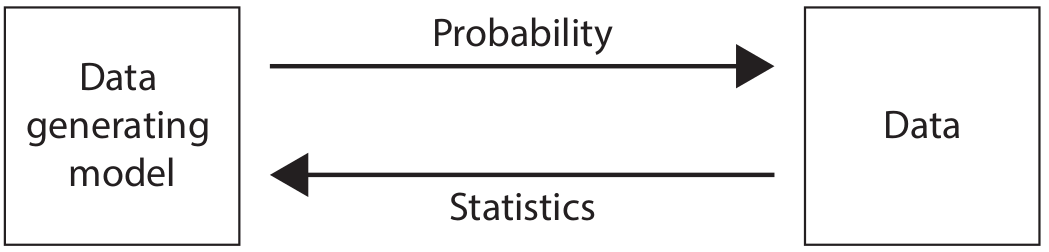
\includegraphics[width=0.7\linewidth]{cartoon.png}
	\end{figure}

\end{frame}

\begin{frame}{Populations and random samples}

	A \textit{population} is the set of all units or objects one intends to study:
	\begin{itemize}
		\item UK human population (e.g. height)
		\item Human T-lymphotropic Virus-1 (HTLV-1) infected T-cells
		\item Gut microbiota
		\item ...
	\end{itemize}

\end{frame}

\begin{frame}{Populations and random samples}

	Although we would like to study the whole population, observing all the
	units in the population is often not possible:
	\begin{itemize}
		\item Measurement costs are too high (e.g. census)
		\item No access to all units (e.g. online survey respondents, T-cells in a
	blood sample, bacteria in faecal sample)
	\end{itemize}
	
	\begin{block}{}
		A \textit{random sample} is a subset of the population that is representative of
		the population.
	\end{block}

\end{frame}

\begin{frame}{Stages of a statistical analysis}

	There are four broad stages:
	\begin{enumerate}
		\item Select measurement variables
		\item Perform random sampling
		\item Construct one or more statistical models
		\item Perform data analysis:
		\begin{itemize} 
			\item Descriptive statistics
			\item Inferential statistics
		\end{itemize}
	\end{enumerate}

\end{frame}

\begin{frame}{1. Measurement variables}

	The initial stage of any experimental analysis involves the selection of
	variables to observe and their measurement scale.

	\vskip 0.5cm

	There are two types of data:
	\begin{itemize}
		\item Quantitative
		\pause
		\begin{itemize}
			\item Continuous (e.g. concentration) vs. Discrete (e.g. cell counts)
			\item Univariate (e.g. light intensity) vs. Multivariate (e.g. chemotaxis: 2D movement vector, microarray data)
		\end{itemize}
		\item Qualitative
		\pause
		\begin{itemize}
			\item Nominal: No logical ordering (categories, classes, binary data. 
			e.g. healthy/diseased, male/female, smoker/non-smoker, etc)
			\item Ordinal: Codes with logical ordering (e.g. exam grades)
		\end{itemize}
	\end{itemize}

\end{frame}

\begin{frame}{2. Random sampling}

	Most statistical analyses assume the following:
	\begin{itemize}
		\item Extract a random sample of $n$ units
		\item All the measurements are collected in sample data $D = \{x_1, ..., x_n\}$
		\item The elements of $D$ are random realisations of $n$ random variables $\{X_1, ..., X_n\}$
		\item Assume variables are independent and identically distributed (i.i.d)
		\item The underlying probability function or density function is $f_X(x) \equiv f_X(x; \theta)$ where $\theta$ is a 
		parameter or parameter vector. 
	\end{itemize}

\end{frame}

\begin{frame}{3. Statistical models}

	\begin{block}{}
		A \textit{statistical model} is a set $\{f_X(x;\theta)| \theta \in \Theta\}$ of probability measures,
	one of which corresponds to the true, unknown, probability measure $p(x; \theta^*)$ that produced the data.
	\end{block}
	$\theta$ is the parameter of the model, and $\Theta$ is the parameter space.

	\pause
	\small

	\begin{itemize}
		\item $\theta^*$ is the true or population parameter such that $p(x; \theta^*)$ is the true probability measure for the data.
		\item We decide on the appropriate model either by using prior knowledge of the data generating process or by using exploratory  statistical tools.
		\item The data space $\mathcal{X}$ and parameter space $\Theta$ are related by different spaces!
	\end{itemize}

\end{frame}

\begin{frame}{4. Data analysis}

	\begin{itemize}
		\item \textit{Descriptive statistics} is the discipline of summarising and describing data (e.g. quantitative summaries and 
	visual representations of the data)
		\item \textit{Inferential statistics} is the branch of statistics which attempts to draw conclusions about the the population from random samples
	\end{itemize}

\end{frame}

\section{Descriptive statistics}

\begin{frame}{Descriptive statistics: summaries of the data}

	Given a random sample, one produces numerical and visual summaries of the data in order to:
	\begin{itemize}
		\item Detect trends or features in the observed data
		\item Detect outliers
		\item Suggest appropriate statistical models, often in the absence of prior knowledge (e.g. bi-modality in histograms suggests mixture models)
	\end{itemize}	

	Typical quantitative summaries of data fall into several classes: location or central tendency measures,
	mode, scale (or spread of the data), skewness (or asymmetry).

\end{frame}

\begin{frame}{Central tendencies}

	\begin{itemize}
		\item arithmetic mean (or sample mean)
		\item weighted arithmetic mean
		\item geometric mean
		\item harmonic mean
	\end{itemize}

\end{frame}

\begin{frame}{Central tendencies}
	\begin{figure}
		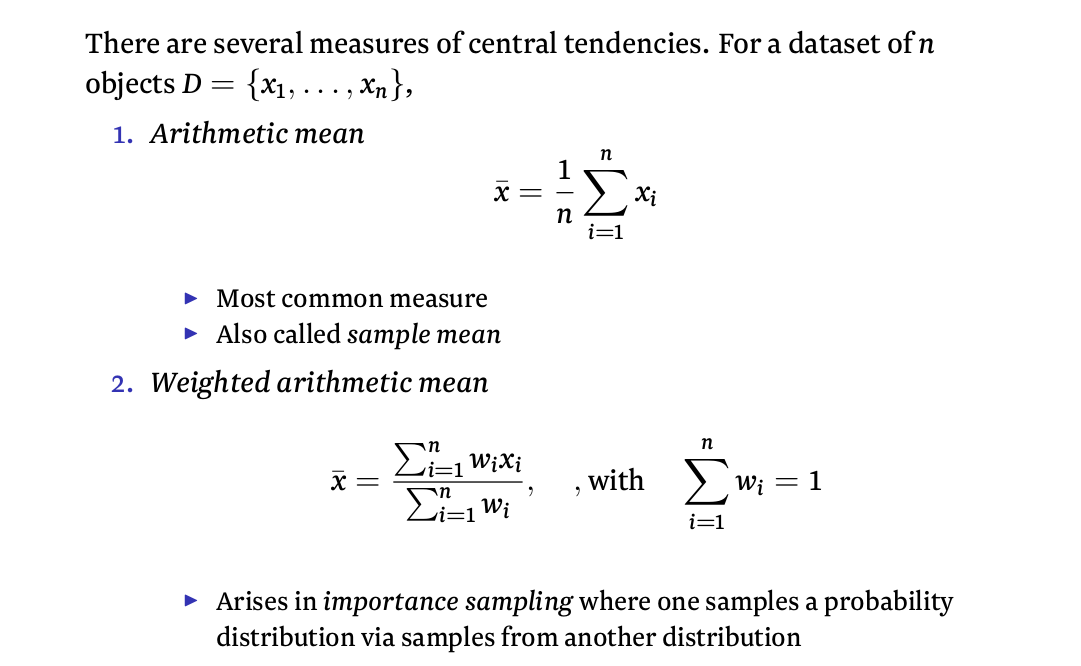
\includegraphics[width=0.9\linewidth]{mean1.png}
	\end{figure}
\end{frame}

\begin{frame}{Central tendencies}
	\begin{figure}
        	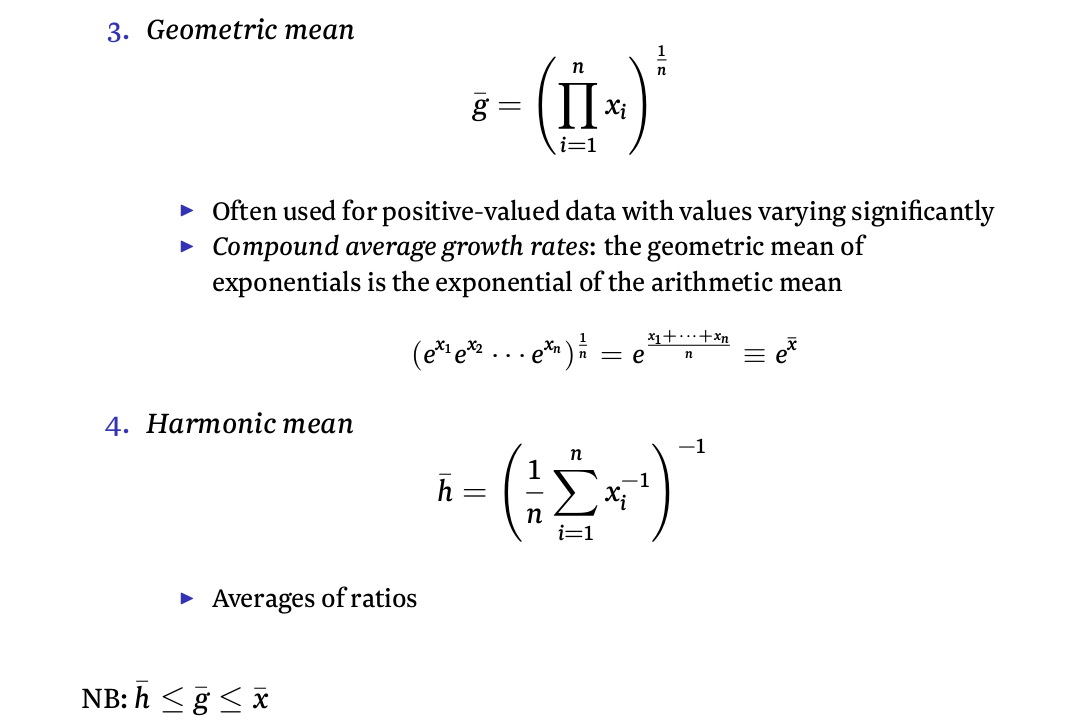
\includegraphics[width=0.8\linewidth]{mean2.png}
	\end{figure}
\end{frame}

\begin{frame}{Scale}

	For univariate sample data, the common summary measures for scale are
	\begin{itemize}
		\item sample minimum
		\item sample maximum
		\item sample range
		\item $p^{th}$-quantile of the empirical distribution function: median, lower and upper quartiles, inter-quartile range.
		\item (unbiased) sample variance
		\begin{equation*}
			s_{n-1}^2 = \frac{1}{n-1} \sum_{i=1}^n (x_i - \hat{x})^2
		\end{equation*}
	\end{itemize}

\end{frame}

\begin{frame}{Skewness}

	Third and higher moments of a distribution can provide useful descriptions.

	Skewness measures the departure from symmetry of the probability distribution of a real-valued random variable.

	\begin{figure}
		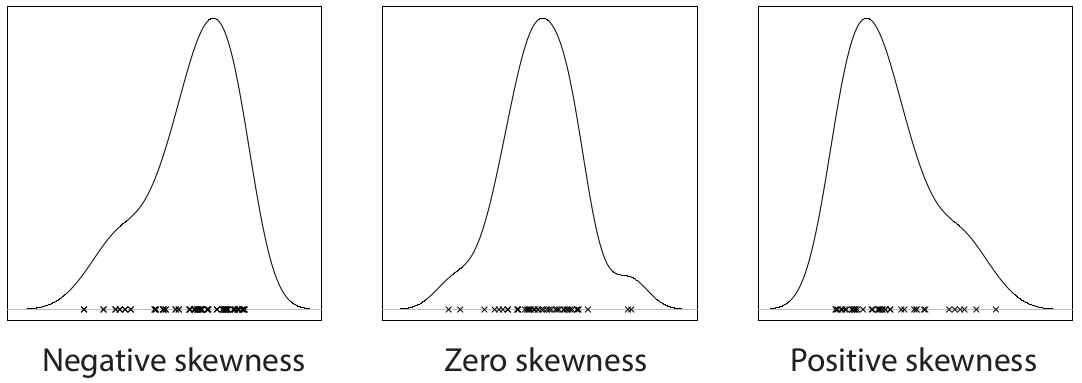
\includegraphics[width=0.9\linewidth]{skew.png}
	\end{figure}

\end{frame}

\begin{frame}{Graphical summaries}

	In addition to the preceding quantitative summaries, it is often useful to
	provide visual or graphical summaries.

	\begin{itemize}
		\item The type of graphs/plots depend on the data obtained, e.g. Discrete or continuous, Uni- or multivariate.
		\item Besides providing a summary of the data, graphical summaries can also illustrate any testing we may wish to perform.
	\end{itemize}

\end{frame}

\begin{frame}{Discrete data visualisation - Barplot and piecharts}

	\begin{figure}
                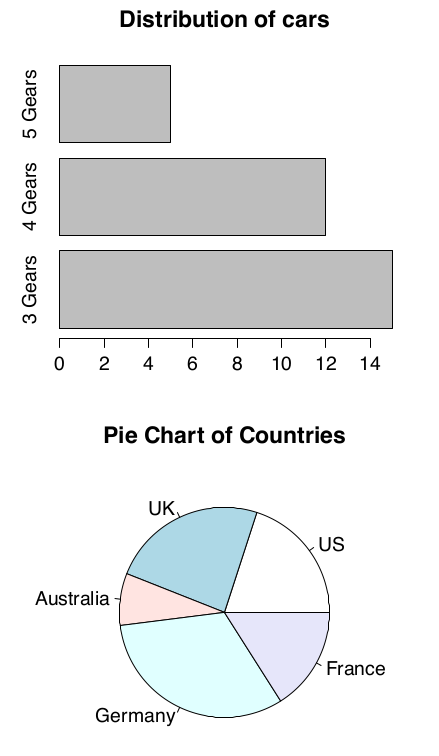
\includegraphics[width=0.3\linewidth]{barplot.png}
        \end{figure}

\end{frame}

\begin{frame}{Continuous data visualisation – Histograms and density estimates}

        \begin{figure}
                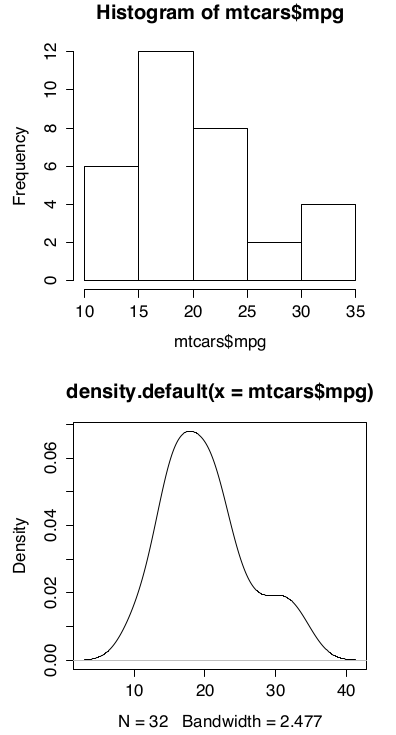
\includegraphics[width=0.3\linewidth]{histogram.png}
        \end{figure}

\end{frame}

\begin{frame}{Continuous data visualisation – Boxplots}

        \begin{figure}
                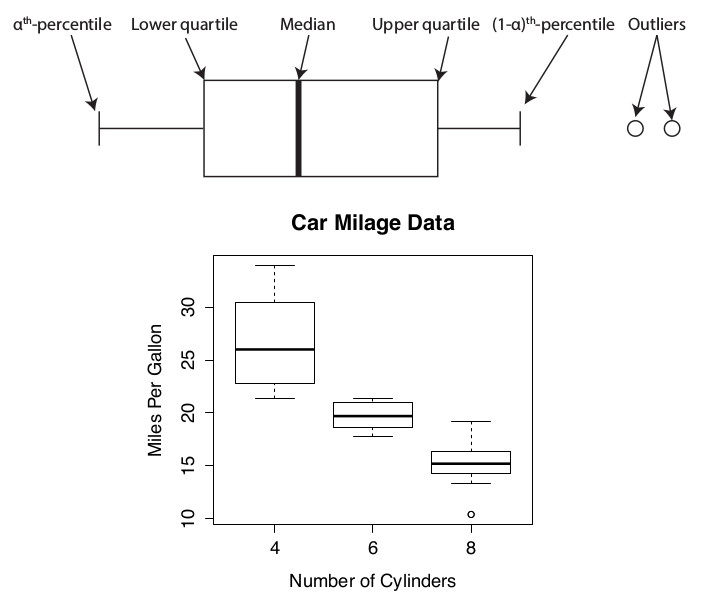
\includegraphics[width=0.7\linewidth]{boxplot.png}
        \end{figure}

\end{frame}

\begin{frame}{Bivariate data visualisation – Scatterplots}

	\begin{figure}
                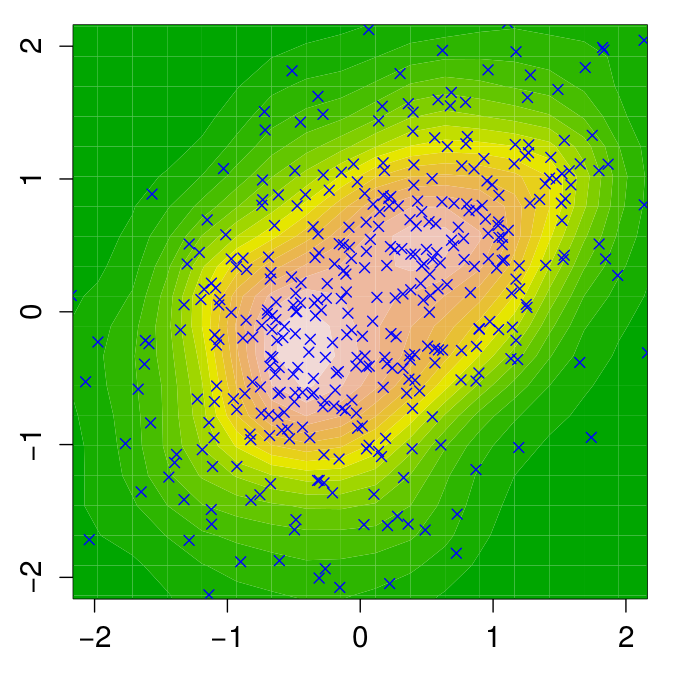
\includegraphics[width=0.5\linewidth]{scatter.png}
        \end{figure}

\end{frame}

\begin{frame}{Probability plotting techniques - QQ plot}

        \begin{figure}
                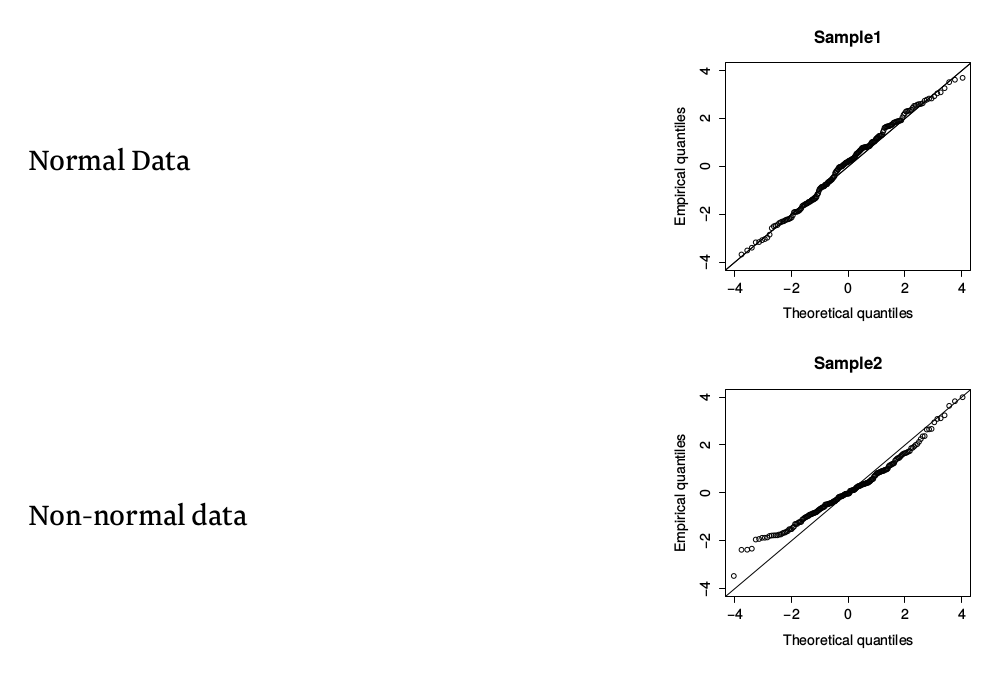
\includegraphics[width=0.8\linewidth]{qqplot.png}
        \end{figure}

\end{frame}

\section{Inferential statistics}

\begin{frame}{Inferential statistics}

        It provides the mathematical theory for inferring properties of an unknown distribution
        from data generated from that distribution.

        \begin{itemize}
                \item In the \textit{parametric} approach, one selects a suitable distribution and attempt to infer the parameters from the data.
                \item In a \textit{non-parametric} approach, one does not make any assumption about the underlying distribution of the data.
        \end{itemize}

        There are several approaches to statistical inference: frequentist, likelihoodist, Bayesian.

\end{frame}

\begin{frame}{Statistical inference}

	Assume that we know and accept a statistical model $f_X(x; \theta)$.

	\begin{block}{}
		The main objective of parametric statistical inference is to learn
		something about the unknown population parameter $\theta$ from
		information contained in sample data.
	\end{block}

	We will use an estimator or \textit{statistic}, a function of the sample data,  to
	learn about $\theta$.
	
\end{frame}

\begin{frame}{Statistical inference}

	Common tasks are:
	\begin{enumerate}
		\item Point estimation: obtain a single estimate $\hat{\theta}$ of the population parameter $\theta$
		\item Interval estimation: obtain an interval having a certain probability
		to contain the unknown population parameter $\theta$
		\item Hypothesis testing: test a specific hypothesis about $\theta$, i.e. do the
		observed data support the hypothesis?
	\end{enumerate}

\end{frame}

\begin{frame}{Estimators}

	An estimator or statistic is a function of the random sample $D=\{x_1,...,x_n\}$, say $t(D)$.

	\begin{itemize}
		\item $t(D)$ depends on the data sample alone
		\item We have already encountered several statistics, e.g. the sample mean and the sample variance
		\item Because an estimator is a function of random variables, it is itself a
		random variable with its own distribution. We usually refer to the
		latter as the \textit{sampling distribution of the sample statistic}.
	\end{itemize}

\end{frame}

\begin{frame}{Estimators}

	Estimators are used to estimate the unknown population parameters.

	\vskip 0.5cm

	For instance, if we assume some parametric model with population mean parameter $\mu$, 
	we may want to use $\hat{x}$ as an estimate for $\mu$.

	\vskip 0.5cm

	Often, it is not trivial to construct estimators. One approach is the maximum likelihood estimator (more on this later).

\end{frame}

\begin{frame}{Constructing and characterising estimators}

	We encountered several measures of central tendency – the (arithmetic) sample mean, median, geometric mean, etc.

	\begin{block}{}
	Which estimator is the "best" one for estimating the population mean parameter $\theta$? 
	How is one estimator "better" than another?
	\end{block}

	\pause

	\begin{itemize}
		\item Since estimators are random variables, we compare them by assessing their
		respective sampling distribution (when known)
		\item We will look at the following properties: 1. Bias, 2. Mean Squared
		Error (MSE), 3. Efficiency, 4. Consistency
	\end{itemize}

\end{frame}

\begin{frame}{Bias}

	\begin{itemize}
		\item Suppose we could repeat the same experiment a number of times, say $B$, and collect new data $D$ each time.
		\item Each time we use our estimator $t(D)$ of choice to obtain an estimate $\hat{\theta}$ of an unknown 
	population parameter $\theta$.
		\item We have a set of different estimates which are of samples from the sampling distribution of the
	estimator/sample-statistic $t(D)$.
	\end{itemize}

	\pause
	
	The bias of an estimator $t(D)$ is defined as
	\begin{equation*}
		bias(t(D)) = E_\theta(t(D)) - \theta
	\end{equation*}

	An \textit{unbiased} estimator is one with zero bias, i.e. $E_\theta(t(D)) = \theta$.

	\tiny
	jupyter-notebook: inference

\end{frame}

\begin{frame}{Mean squared error (MSE) and standard error of an estimate}
	
	How much variability do we expect to see in $\hat{\theta}$ under repeated sampling from the 
	assumed distribution?

	\vskip 0.5cm

	\pause

	A common measure of the spread of the sampling distribution $t(D)$ around the true parameter $\theta$ is given by 
	the mean squared error (MSE)
	\begin{equation*}
		MSE(t(D)) = E{(t(D)-\theta)^2}
	\end{equation*}

	It measures the average \textit{spread} difference between the estimator and $\theta$.

\end{frame}

\begin{frame}{Mean squared error (MSE) and standard error of an estimate}

	The MSE has two components:
	\begin{itemize}
		\item the variability of the estimator (precision)
		\item its bias (accuracy)
	\end{itemize}

	\vskip 0.5cm

	For an unbiased estimator, the MSE equal its variance and the standard error is the square root of the MSE.

\end{frame}

\begin{frame}{Efficiency}

	All things equal, we choose the unbiased estimator with the smallest variance, i.e. with higher precision.

	\vskip 1cm

	The efficiency of $t_1(D)$ relative to $t_2(D)$ is
	\begin{equation*}
		efficiency = \frac{Var(t_2(D))}{Var(t_1(D))}
	\end{equation*}

\end{frame}

\begin{frame}{Consistency}

	Consistency is an asymptotic property of an estimator.

	\vskip 0.5cm

	It describes the behaviour of the estimator $t(D)$ as the sample size $n$ gets
	larger and larger. Hence it involves a sequence of estimators.

	\vskip 0.5cm

	Two sufficient conditions for consistency are:
	\begin{itemize}
		\item $ \lim_{n \rightarrow \infty} E(t_n)=\theta $
		\item $ \lim_{n \rightarrow \infty} Var(t_n)=0 $
	\end{itemize}

\end{frame}

\begin{frame}{Wrap up}

	\begin{enumerate}
		\item Stages of a statistical analysis:
			\begin{enumerate}
				\item Define measurement variables
				\item Perform random sampling 
				\item Choose a statistical model
				\item Perform data analysis
			\end{enumerate}
		\item Descriptive statistics
			\begin{itemize}
				\item data summaries
				\item visualisation
			\end{itemize}
		\item Statistical inference
			\begin{itemize}
				\item estimators and their properties
				\item ...
			\end{itemize}
	\end{enumerate}

\end{frame}

\section{Likelihood}

\begin{frame}{Model fitting}

	How do we fit models to data? A model will have one or more 
	parameters, $\theta$, that we need to estimate to get a good fit.

	\begin{figure}
		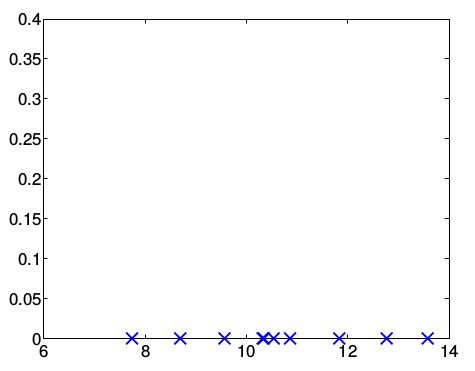
\includegraphics[width=0.4\linewidth]{fit1.png}
	\end{figure}

	e.g. we may want to model some observations as being normally
	distributed with mean $\mu$ and standard deviation 1.
	\begin{center}
		What is $\mu$?
	\end{center}

\end{frame}

\begin{frame}{Model fitting}

	\begin{center}
                What is $\mu$?
        \end{center}

        \begin{figure}
                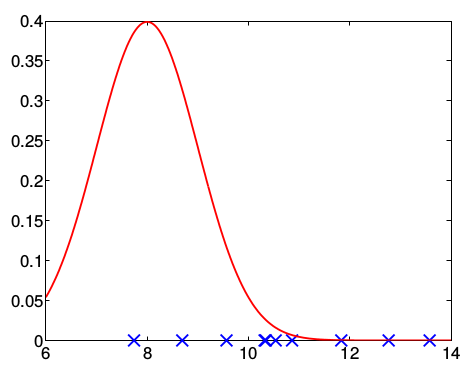
\includegraphics[width=0.4\linewidth]{fit2.png}
        \end{figure}

        $\mu=8$?

\end{frame}

\begin{frame}{Model fitting}

	\begin{center}
                What is $\mu$?
        \end{center}

        \begin{figure}
                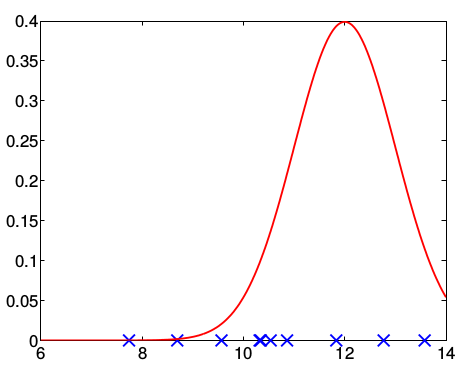
\includegraphics[width=0.4\linewidth]{fit3.png}
        \end{figure}

        $\mu=12$?

\end{frame}

\begin{frame}{Model fitting}

	\begin{center}
                What is $\mu$?
        \end{center}

        \begin{figure}
                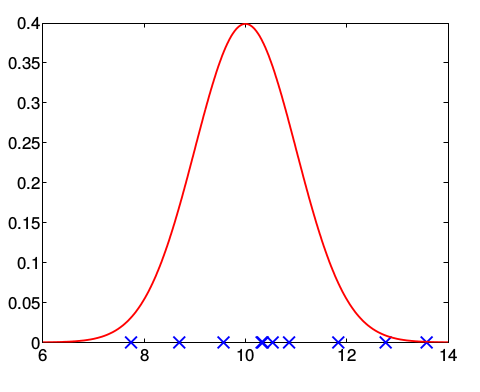
\includegraphics[width=0.4\linewidth]{fit4.png}
        \end{figure}

        $\mu=10$?

\end{frame}

\begin{frame}{Likelihood}

	\begin{itemize}
		\item The concept of likelihood provides us with a formal framework for
			estimating parameters.
		\item In particular, maximum likelihood estimation is a general method
			for estimating the parameters of a (probability) model.
		\item The likelihood function is also one of the key ingredients for
Bayesian inference.
	\end{itemize}

\end{frame}

\begin{frame}{Likelihood}

        \begin{figure}
                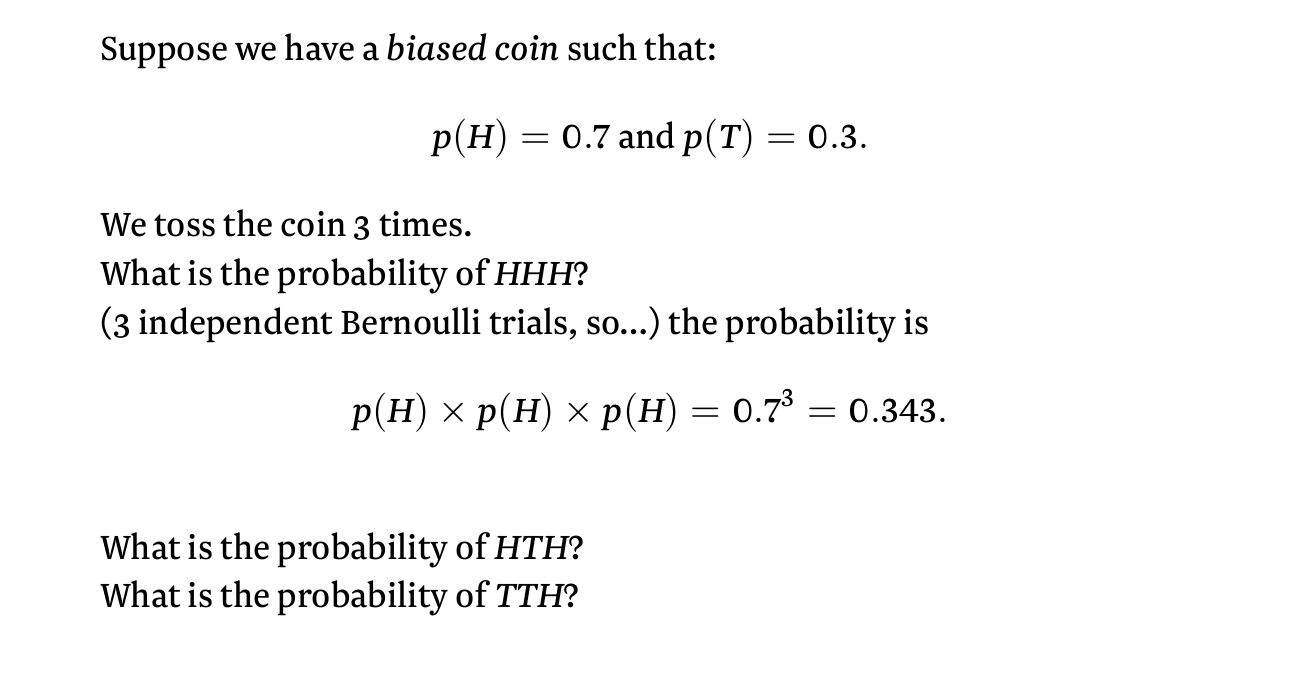
\includegraphics[width=\linewidth]{like1.png}
        \end{figure}

\end{frame}

\begin{frame}{Likelihood}

        \begin{figure}
                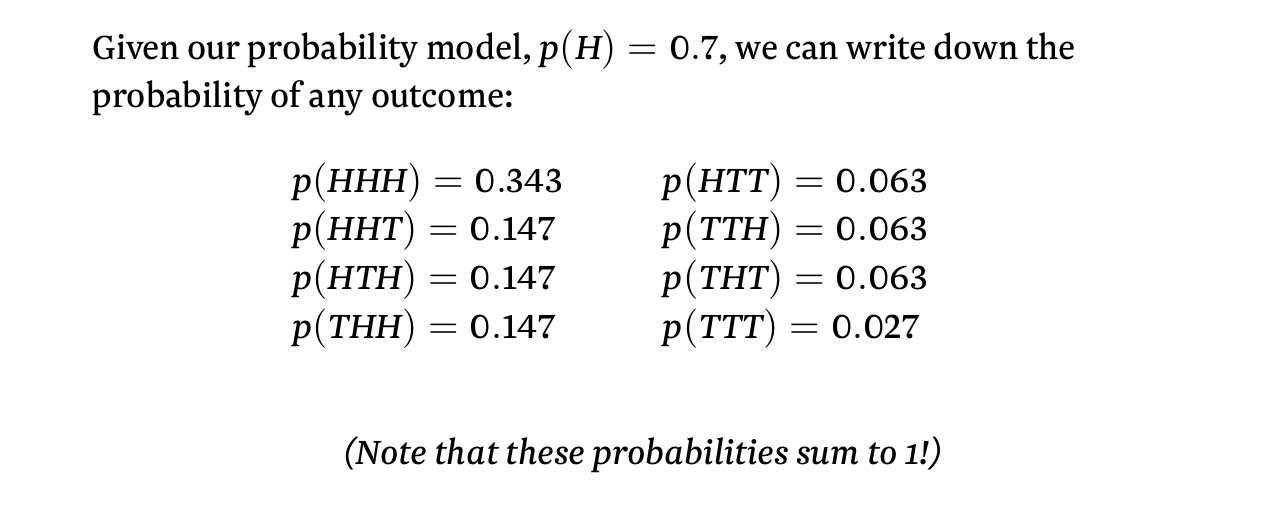
\includegraphics[width=\linewidth]{like2.png}
        \end{figure}

\end{frame}
\begin{frame}{Likelihood}

        \begin{figure}
                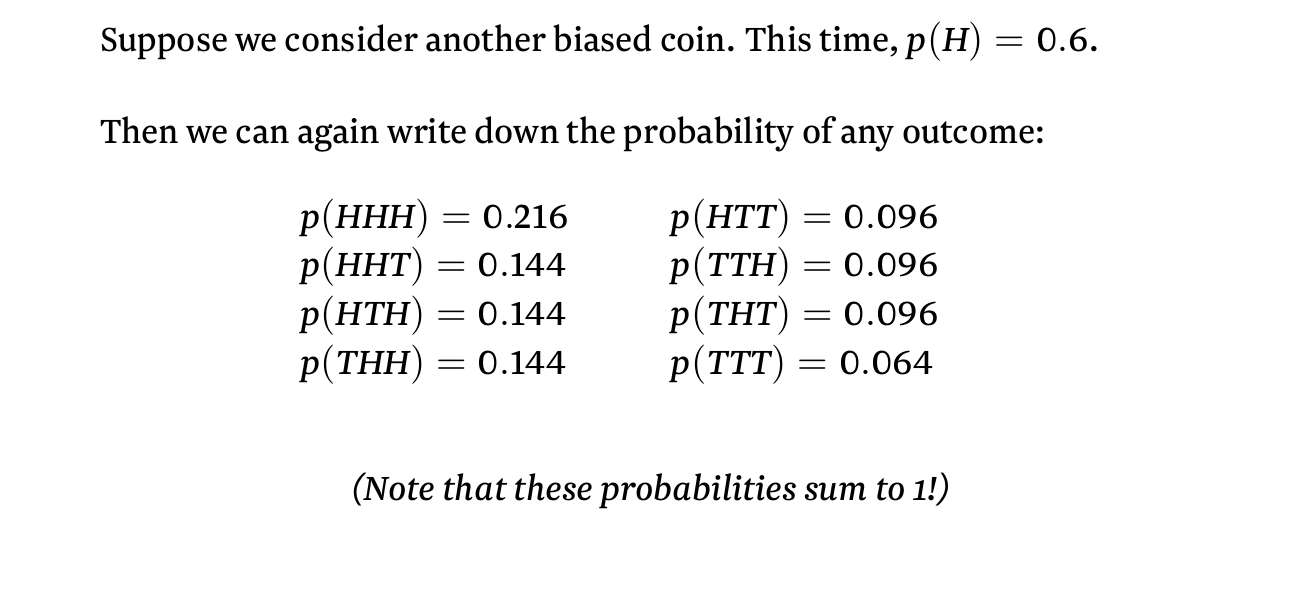
\includegraphics[width=\linewidth]{like3.png}
        \end{figure}

\end{frame}
\begin{frame}{Likelihood}

        \begin{figure}
                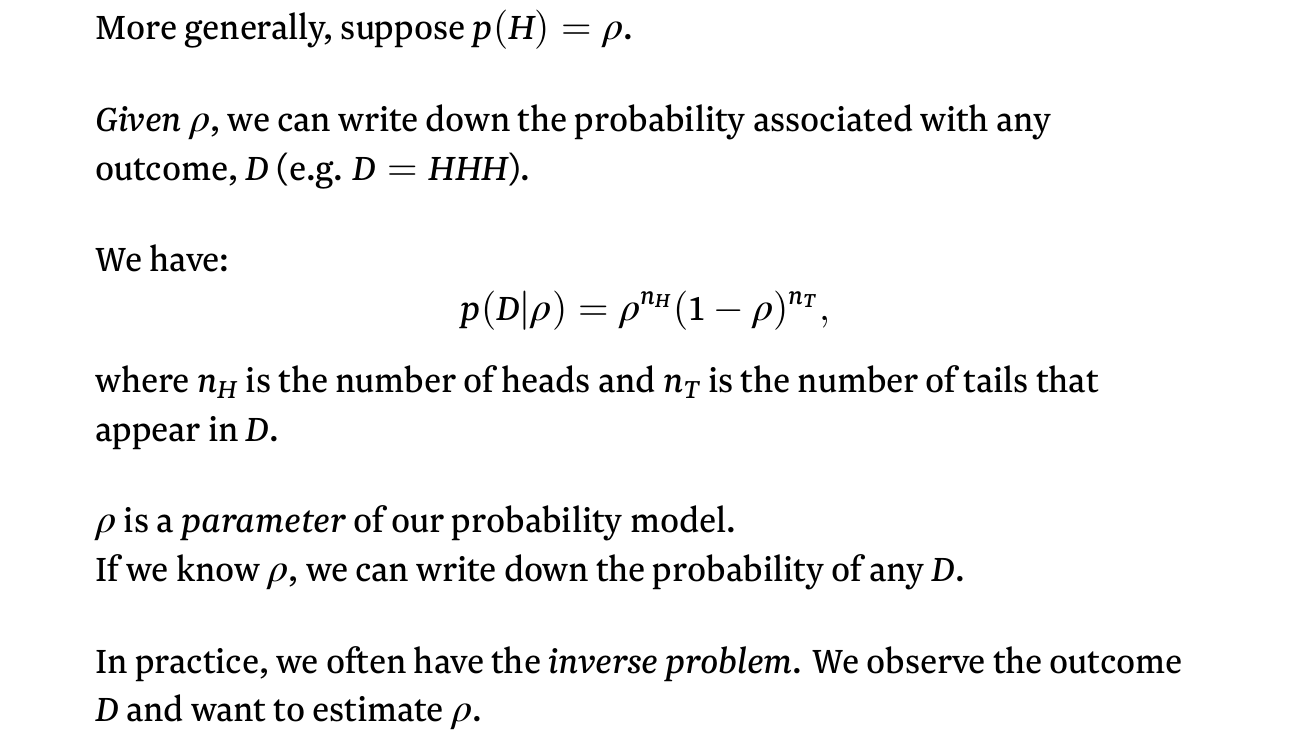
\includegraphics[width=\linewidth]{like4.png}
        \end{figure}

\end{frame}
\begin{frame}{Likelihood}

        \begin{figure}
                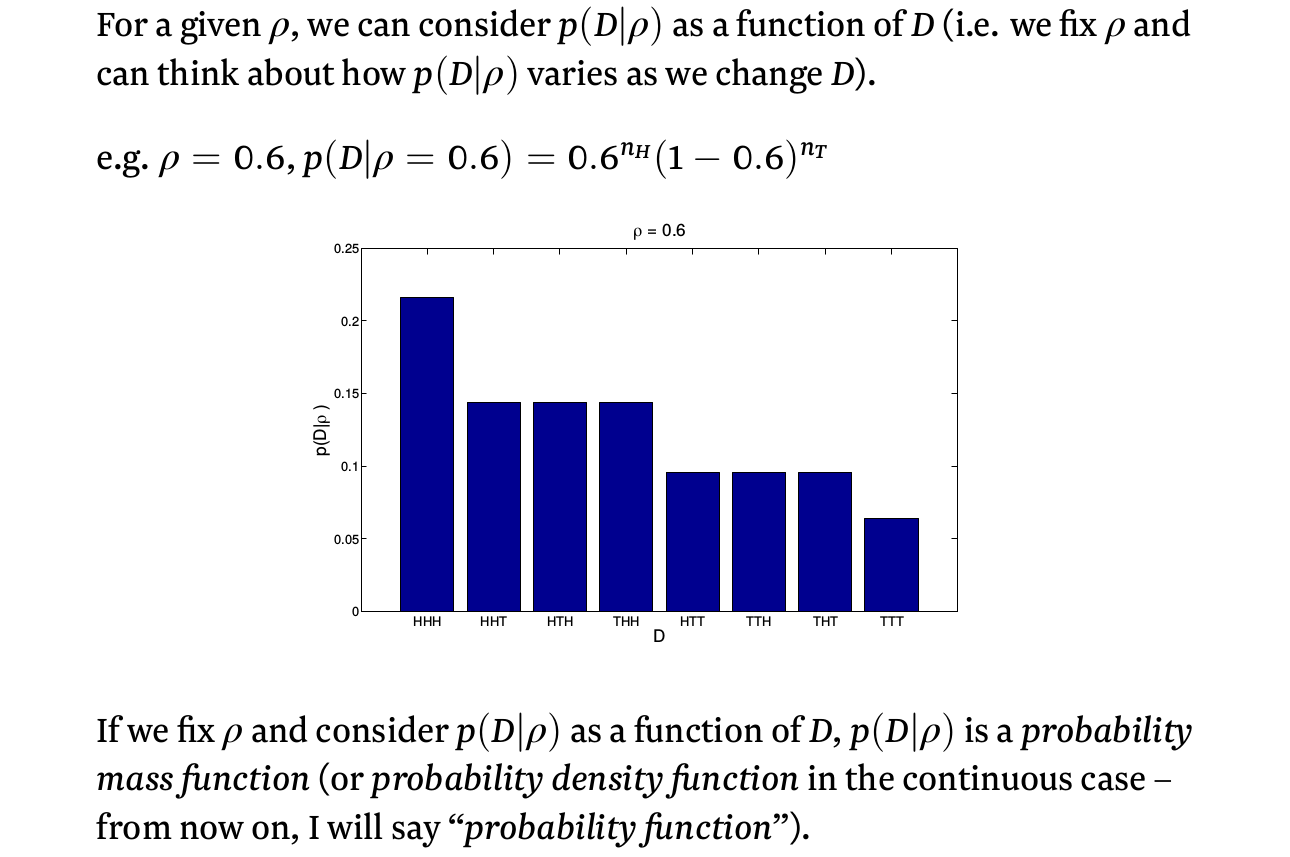
\includegraphics[width=\linewidth]{like5.png}
        \end{figure}

\end{frame}
\begin{frame}{Likelihood}

        \begin{figure}
                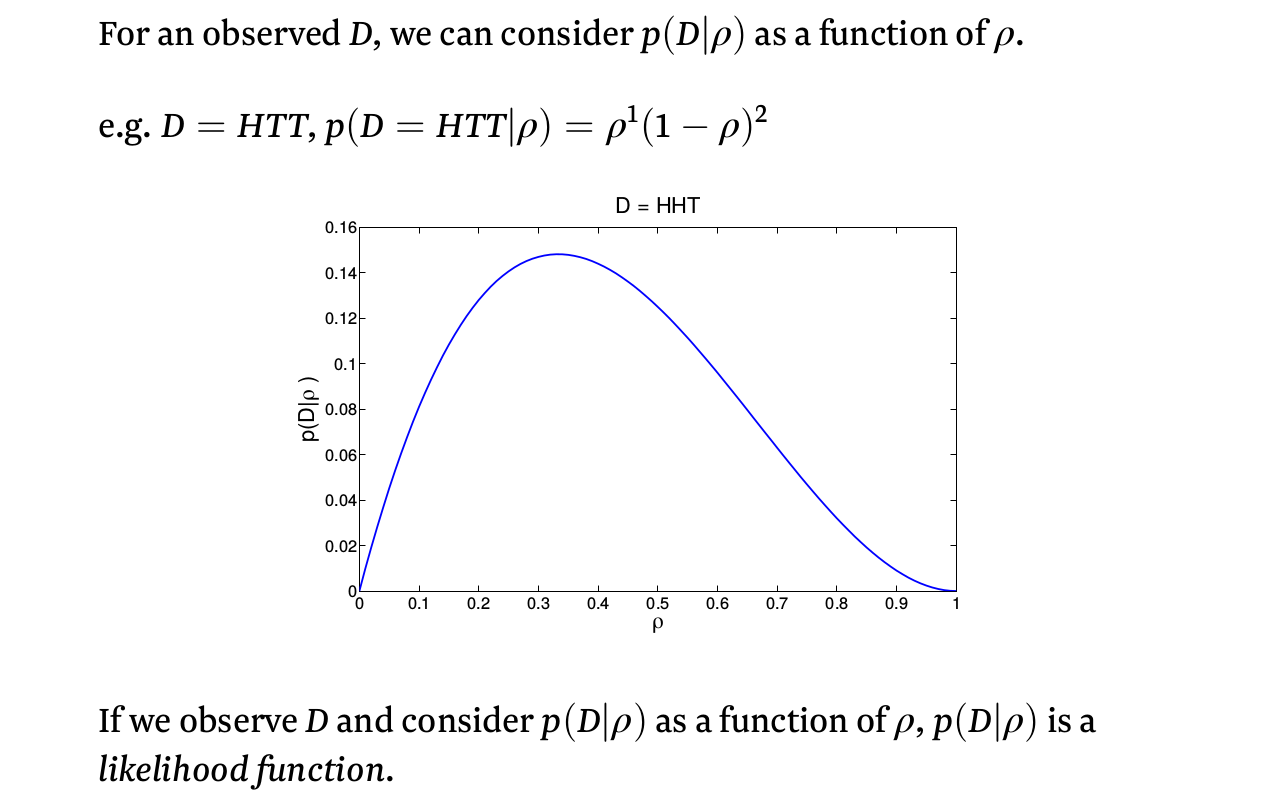
\includegraphics[width=\linewidth]{like6.png}
        \end{figure}

\end{frame}
\begin{frame}{Likelihood}

        \begin{figure}
                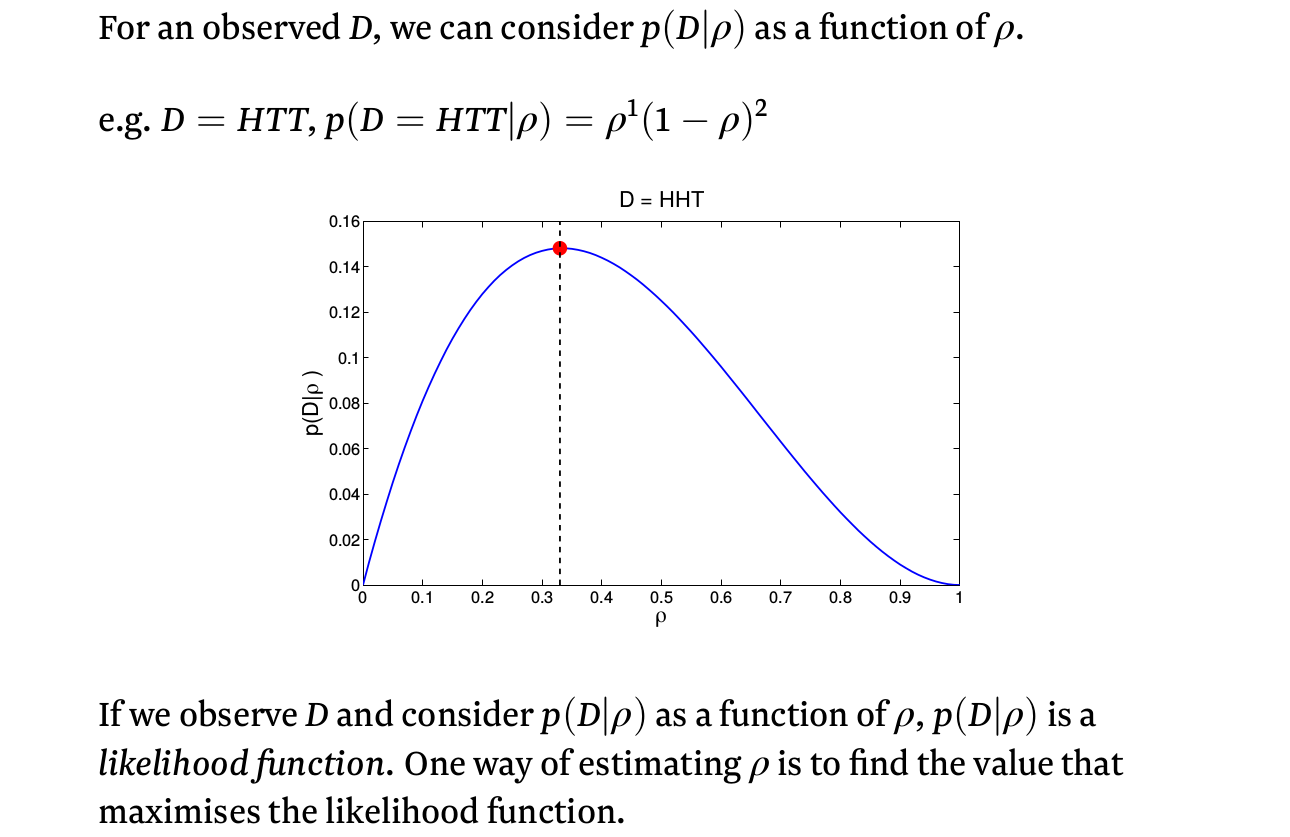
\includegraphics[width=\linewidth]{like7.png}
        \end{figure}

\end{frame}

\begin{frame}{Likelihood}

        \begin{figure}
                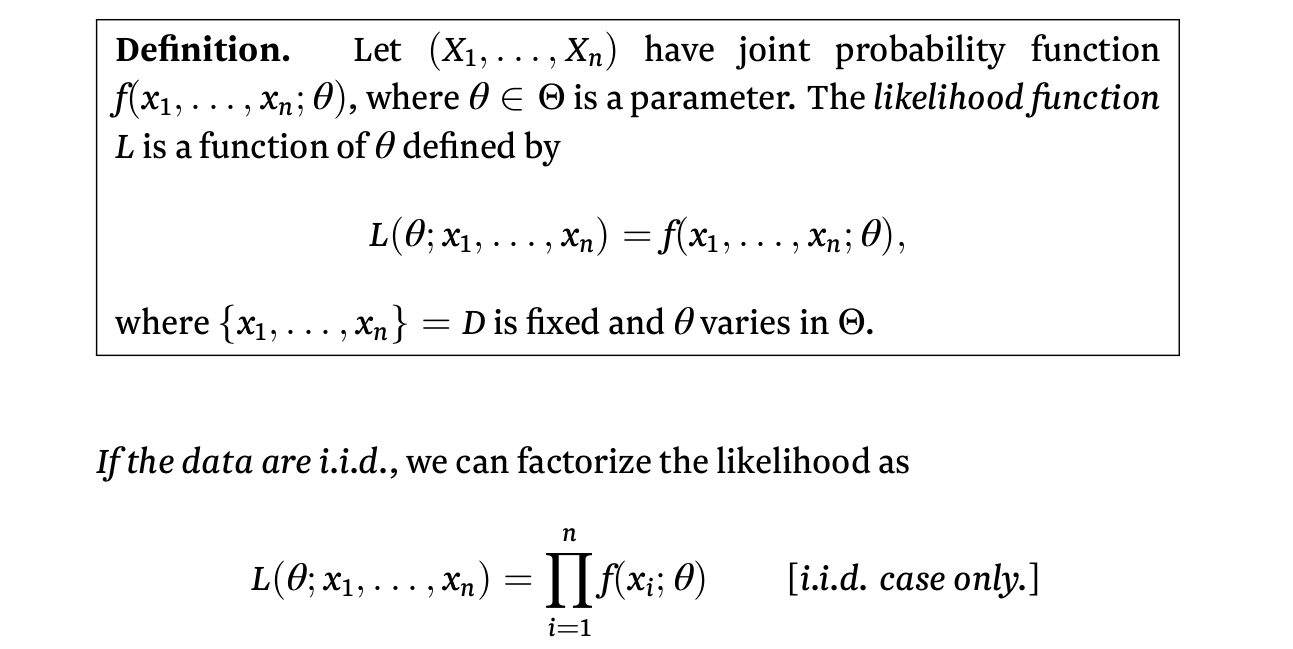
\includegraphics[width=\linewidth]{like8.png}
        \end{figure}

\end{frame}

\begin{frame}{Maximum likelihood estimate}

        \begin{figure}
                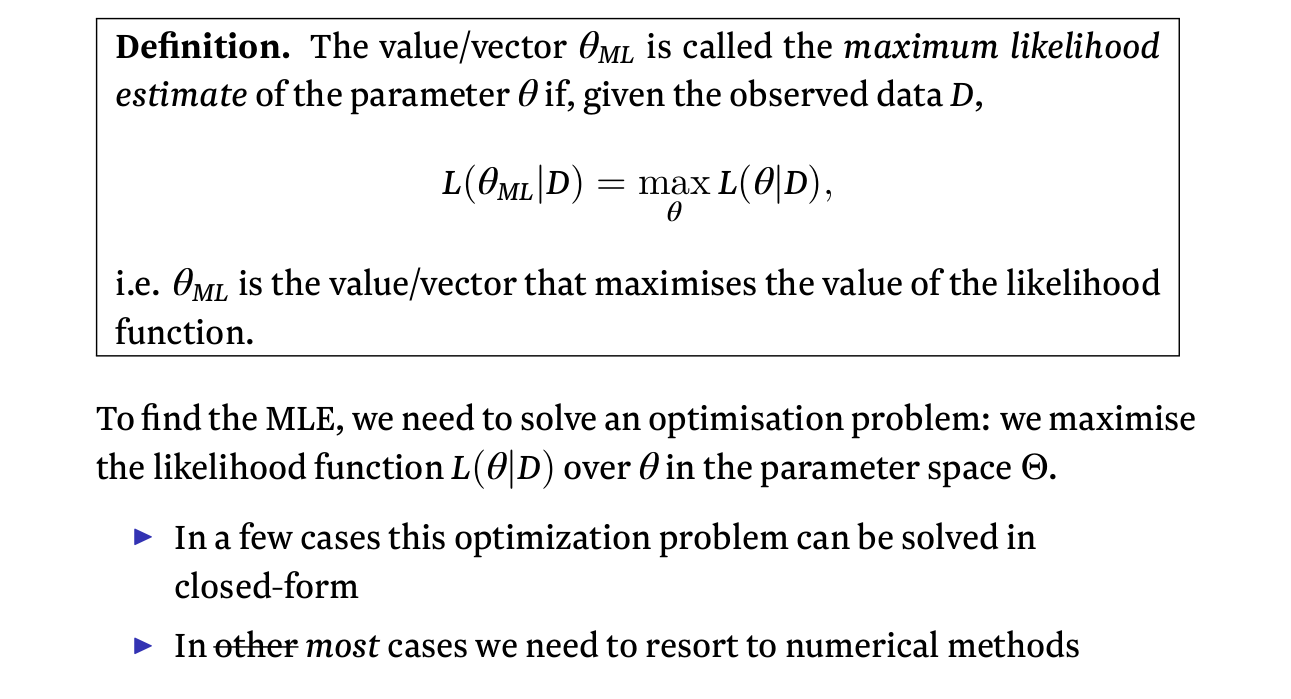
\includegraphics[width=\linewidth]{like9.png}
        \end{figure}

\end{frame}

\begin{frame}{Wrap up}

	\begin{figure}
                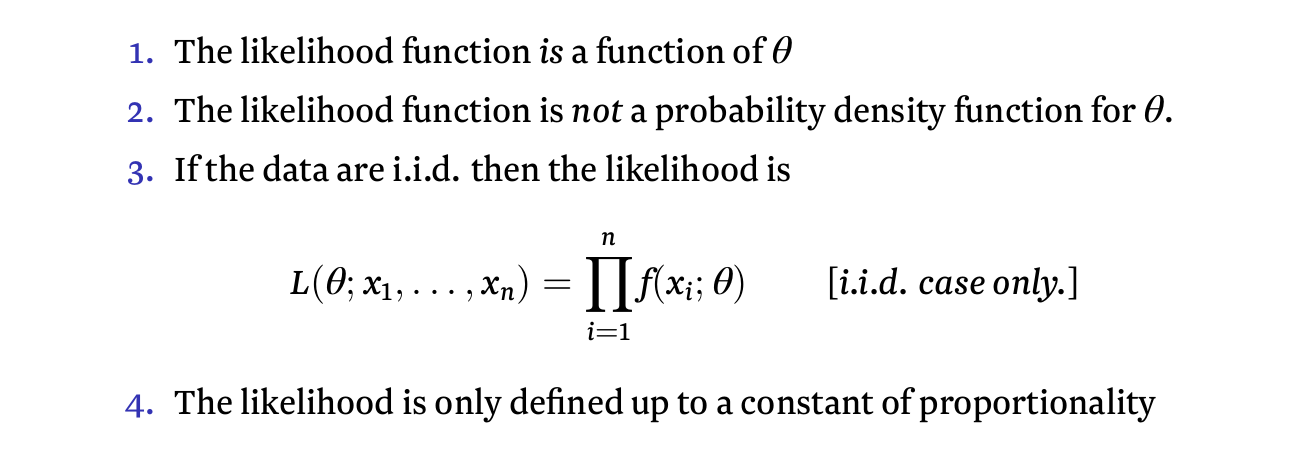
\includegraphics[width=\linewidth]{like10.png}
        \end{figure}

	\tiny
	jupyter-notebook: inference 

\end{frame}

\section{Hypothesis testing}

\begin{frame}{Statistical tests}

	\begin{itemize}
		\item In our study of statistical inference, we have focused on point estimation
	of unknown parameters of a given statistical model.
		\item  The residual uncertainty is expressed as uncertainty in these point
	estimates (e.g. sampling distribution of estimator).
		\item We will now look at \textit{hypothesis testing}
		\begin{itemize}
 			\item Make a definitive hypothesis about $\theta$
			\item Uncertainty is reflected in the expected probability of being wrong (\textit{p}-value)
		\end{itemize}
	\end{itemize}

\end{frame}

\begin{frame}{Statistical test}

	We will encounter a wide range of statistical tests:
	\begin{itemize}
		\item Parametric vs. Non-parametric
		\item One-sided vs. Two-sided tests
		\item Z-test, t-test, goodness-of-fit tests, likelihood ratio test, etc...
	\end{itemize}

	\pause

	However, there is a common approach to all statistical tests:
	\begin{enumerate}	
		\item Generate a Null Hypothesis and an Alternative Hypothesis
		\item Obtain the sampling distribution of the estimator under the null
		hypothesis: the Null distribution
		\item Decide whether to reject the null hypothesis
	\end{enumerate}

\end{frame}

\begin{frame}{Null and Alternative Hypotheses}

	Suppose we want to know if the use of a drug is associated to a symptom.

	\begin{itemize}
	\item We take some mice and randomly divide them into two groups.

	\item We expose one group to the drug and leave the second group unexposed.

	\item We then compare the symptom rate in the two groups, $\theta_1$, $\theta_2$ respectively.
	\end{itemize}

\end{frame}

\begin{frame}{Null and Alternative Hypotheses}

	Consider the following two hypotheses:
	\begin{itemize}
		\item The Null Hypothesis: The symptom rate is the same in the two groups, $H_0:\theta_1 = \theta_2$
		\item The Alternative Hypothesis: The symptom rate is not the same in the two groups, $H_1:\theta_1 \neq \theta_2$
	\end{itemize}

	\vskip 0.5cm

	If the exposed group has a much higher rate of symptom than the
	unexposed group, we will \textbf{reject} the null hypothesis and conclude that
	the data favours the alternative hypothesis.

\end{frame}

\begin{frame}{Null and Alternative Hypotheses}

	Let $\Theta$ be the parameter space of a statistical model. 

	We partition $\Theta$ into two disjoint  sets $\Theta_0$ and $\Theta_1$ and test
	\begin{equation*}
		H_0 = \theta \in \Theta_0 \text{ vs. } H_1 = \theta \in \Theta_1 
	\end{equation*}

	$H_0$ and $H_1$ are the Null and Alternative hypotheses, respectively.

\end{frame}

\begin{frame}{Null and Alternative Hypotheses}

	\begin{itemize}
		\item A hypothesis of the form $\theta = \theta_0$ is called a \textit{simple} hypothesis.
		\item A hypothesis of the form $\theta > \theta_0$ (or $\theta < \theta_0$ ) is called a \textit{composite} hypothesis.
	\end{itemize}

	\vskip 0.5cm

	\begin{itemize}
		\item A test of the form $H_0: \theta = \theta_0 \text{ vs. } H_1: \theta \neq \theta_0$ is called a
	\textit{two-sided test}.
		\item A test of the form $H_0: \theta = \theta_0 \text{ vs. } H_1:\theta < \theta_0$ (or $>$) is called a \textit{one-sided test}.
	\end{itemize}

\end{frame}

\begin{frame}{The Null distribution}

	Let $D$ be a random sample of data.

	We test a hypothesis by finding a set of outcomes $R$ called the
	\textit{rejection} region. 

	\begin{itemize}
		\item If $D \in R$ we reject the null hypothesis in favour of the alternative hypothesis
		\item if $D \not\in R$, we fail to reject $H_0$
	\end{itemize}

	Can we ever accept $H_0$? \pause No!

\end{frame}

\begin{frame}{The Null distribution}

	$R$ can be in the form $R=\{D:t(D)>c\}$ where $D$ is the data, $t(D)$ is the test statistic, 
	and $c$ is the \textit{critical value(s)}.

	\vskip 0.5cm
	
	The critical value is determined from two things:
	\begin{itemize}
		\item The null distribution, i.e. the sampling distribution of $t(D)$, assuming the null hypothesis is true.
		\item The significance level $\alpha$ (typically $\alpha <<1$).
	\end{itemize}

\end{frame}

\begin{frame}{Significance and confidence intervals}

	\begin{itemize}
		\item When there is enough evidence to reject $H_0$ , we say that the result
		from a statistical test is "statistically significant at the given
		significance level $\alpha$".
		\item The significance level $\alpha$ controls how stringent the test is. 
		\item When $\alpha$ is very small, the acceptance region is larger and the test is
		more stringent because the null hypothesis will be rejected less frequently.
		\item The probability of making an error and wrongly rejecting the null
		hypothesis when it is in fact true is exactly $\alpha$.
	\end{itemize}

\end{frame}

\begin{frame}{Significance and confidence intervals}

	\begin{block}{}
		\textit{Statistical} significance does not imply \textit{scientific} significance!
	\end{block}

	\vskip 1cm

	It is often more informative to give \textit{confidence intervals}.
	
	A $(1 - \alpha)$-confidence interval (C.I.) is an interval in which the true
	parameter lies with probability $1 - \alpha$.
	
\end{frame}

\begin{frame}{p-values}

	We have established a decision rule: we reject $H_0$ when the value of the
	test statistic falls outside the acceptance region.

	Other than a reject/accept decision, the result of a statistical test is often
	reported in terms of a \textit{p}-value.

	\vskip 0.5cm
	
	A \textit{p}-value is
	\begin{itemize}
		\item the probability, under the null hypothesis, of a result as or more
		extreme than that actually observed.
		\item the smallest significance level at which the null hypothesis would be rejected.
	\end{itemize}

\end{frame}

\begin{frame}{p-values}

	A \textit{p}-value is NOT the probability that the null hypothesis is true. i.e. do not confuse
	the \textit{p}-value with $P(H_0 |D)$.

	\vskip 1cm

	A large \textit{p}-value can occur for two reasons:\\ 
	(i) $H_0$ is true or \\
	(ii) $H_0$ is false but the test has low power (e.g. too few samples).

\end{frame}

\begin{frame}{Type I and II errors}

	When we test the null hypothesis versus the alternative hypothesis of a
	population parameter, there are four possible outcomes, two of which
	are erroneous:

	\begin{figure}
		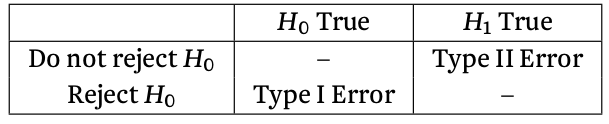
\includegraphics[width=0.6\linewidth]{type.png}
	\end{figure}

	\small
	\begin{itemize}
		\item A Type I error is made when the null hypothesis is wrongly rejected.
		\item A Type II Error is made when we conclude that we do not have enough
evidence to reject the $H_0$ , but in fact the alternative hypothesis $H_1$ is true.
	\end{itemize}

\end{frame}

\begin{frame}{The power of a test}

	The power of a test represents its ability to correctly reject the null
	hypothesis. It is expressed as the probability
	\begin{align*}
		P(\text{Reject }H_0 | H_1 True) &= 1 - P(\text{Do not reject }H_0 | H_1 True) \\
					&= 1 - P(\text{Type II error}) 
	\end{align*}

\end{frame}

\begin{frame}{Statistical tests}

	There are several widely used tests:
	\begin{itemize}
		\item The Wald test: test the true value of the parameter based on the sample estimate.
		\item t-test: to determine if two sets of data are significantly different from each other, assuming normality.
		\item Wilcoxon signed-rank test: non-parametric, to compare two related samples to assess whether their population means are different.
		\item Chi-squared goodness-of-fit test: to test whether observed sample frequencies differ from expected frequencies.
		\item The likelihood ratio test.

	\end{itemize}

\end{frame}

\begin{frame}{Chi-squared goodness-of-fit test}
	\begin{figure}
                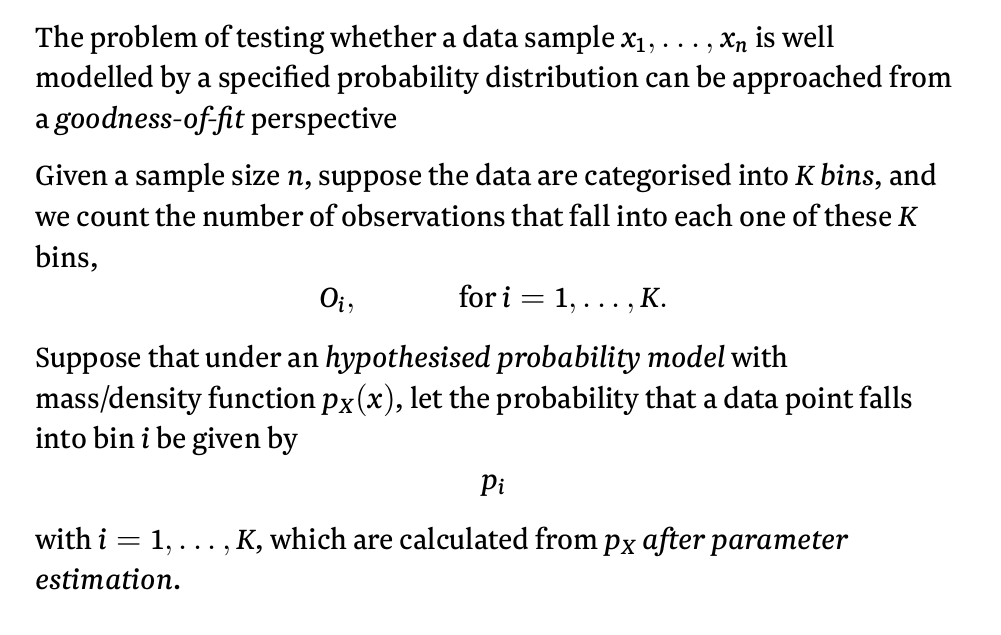
\includegraphics[width=0.85\linewidth]{gof1.png}
        \end{figure}	
\end{frame}

\begin{frame}{Chi-squared goodness-of-fit test}
        \begin{figure}
                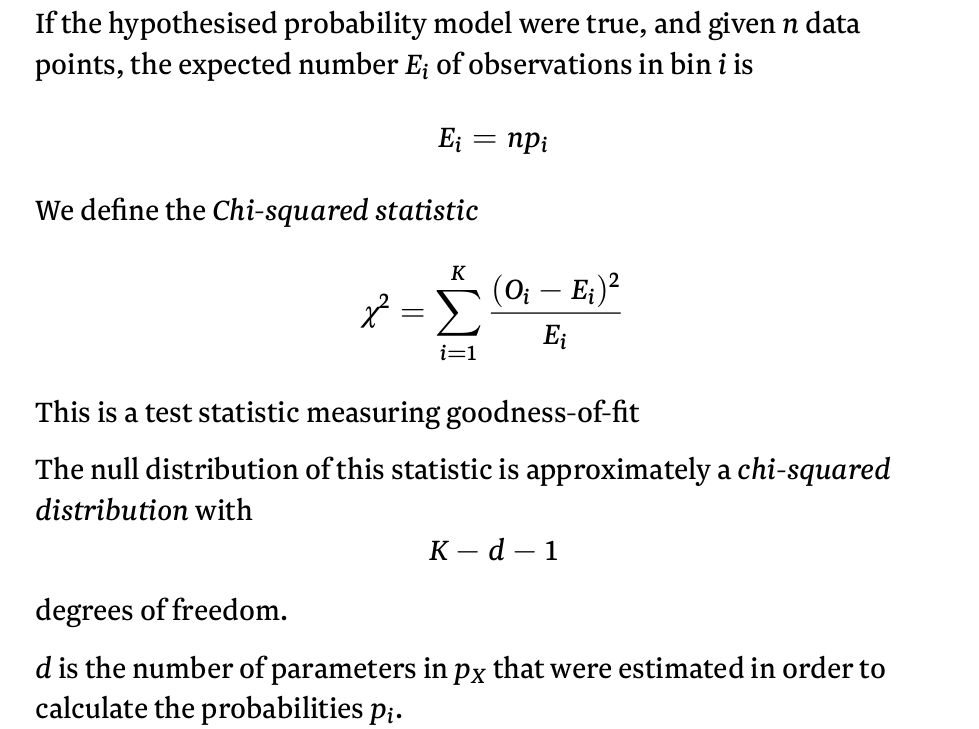
\includegraphics[width=0.85\linewidth]{gof2.png}
        \end{figure}
\end{frame}

\begin{frame}{Chi-squared goodness-of-fit test}

	Example: we observe two alleles, A and G, for a specific genomic locus in a population.
	Specifically, we observe 14 genotypes AA, 4 genotypes AG and 2 genotypes GG.

	\pause

	Can we reject the hypothesis of Hardy Weinberg Equilibrium (HWE, i.e. random mating and no natural selection) for this locus?

	\small
	Note that, under HWE, we expect the following frequencies for the associated genotypes:
	\begin{itemize}
		\item homozygous $f^2$
		\item heterozygous $2f(1-f)$
		\item homozygous $(1-f)^2$
	\end{itemize}

	\tiny jupyter-notebook: inference

\end{frame}

\begin{frame}{Likelihood Ratio Test}
	\begin{figure}
        	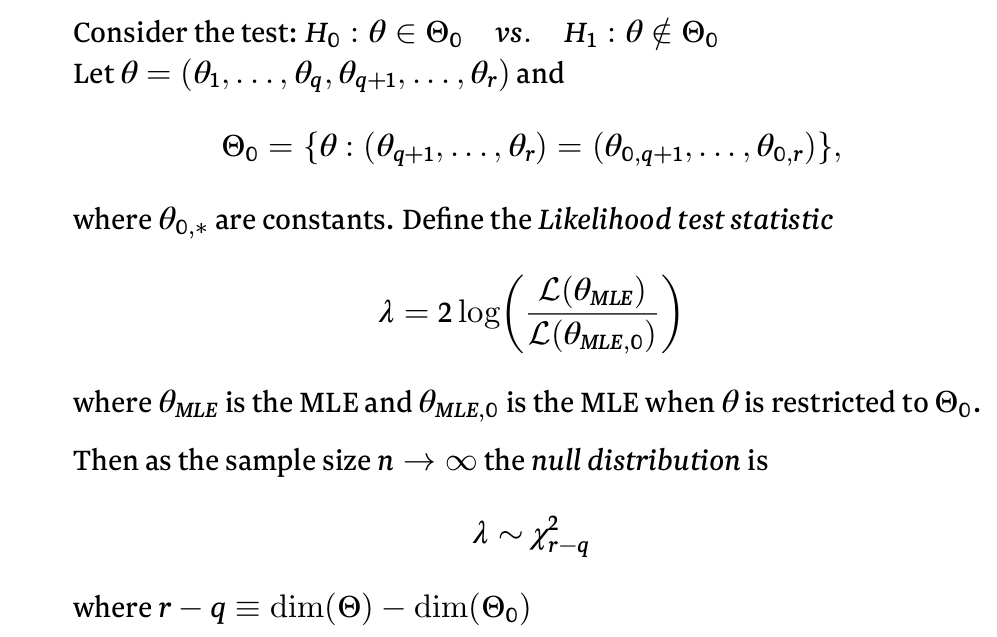
\includegraphics[width=0.85\linewidth]{lrt.png}
	\end{figure}
\end{frame}

\begin{frame}{Bootstrapping}

	It relies on random \textit{sampling with replacement} to assign measure
	of accuracy to sample estimates.

	\vskip 1cm

	The idea is to infer population parameter by resampling the data and performing
	inferences on the sample from the \textit{resampled data}.

	\vskip 1cm

	It assumes that samples are independent (otherwise use block bootstrap for correlated samples).

	\tiny jupyter-notebook: inference

\end{frame}

\begin{frame}{Wrap up}

        General procedure to test statistical hypotheses about a
        population parameter $\theta$:
        \begin{enumerate}
                \item Set up the null and alternative hypotheses for $\theta$, $H_0$ and $H_1$ 
		(one-sided or two-sided).
                \pause
                \item Compute the test statistic and obtain the null distribution, i.e. the
                sampling distribution under the null hypothesis.
                \pause
                \item Choose a significance level $\alpha$ or confidence level $1 - \alpha$.
                \pause
                \item Determine the rejection region for the test statistic, which depends
                on $\alpha$.
                \pause
                \item Apply the decision rule: reject $H_0$ in favour of $H_1$ if the test statistic
                falls in the rejection region. Otherwise conclude that there is
                insufficient evidence to reject $H_0$.
                \pause
                \item Report the \textit{p}-value and construct the confidence interval.
        \end{enumerate}

\end{frame}




\end{document}
